\chapter{PostScript Primer}

%\setcounter{page}{1}

\renewcommand{\thefootnote}{\fnsymbol{footnote}}
\footnotetext{Lecture notes by John Schneider.  {\tt
postscript-primer.tex}}

\section{Introduction}

PostScript was developed by Adobe Systems Incorporated and is both a
page-description language and a programming language.  Unlike a JPEG
or GIF file which says what each pixel in an image should be,
PostScript is ``vector based'' and thus a PostScript file specifies
graphic primitives, such as lines and arcs.  There primitives are
described by various PostScript commands.  The quality of the image
described by a PostScript file will depend on the output device.  For
example, a laser printer with 1200 dots per inch will draw a better
curved line than would a laser printer with 300 dots per inch
(although both will typically produce very good output).

The goal here is to show how one can easily generate PostScript files
which convey information about an FDTD simulation.  Thus we are more
interested in the page-description aspects of PostScript rather than
its programming capabilities.  (There is a wonderful book and Web site
by Bill Casselman that describe PostScript extremely well while
illustrating a host of mathematical concepts.  The book is entitled
{\em Mathematical Illustrations: A Manual of Geometry and PostScript}
which you can find at \url{www.math.ubc.ca/~cass/graphics/manual/}.
It is well worth checking out.)

PostScript is a Forth-like language in that it uses what is known as
postfix notation.  If you have used an RPN (reverse Polish notation)
calculator, you are familiar with postfix notation.  You put arguments
onto a ``stack'' and then select an operation which ``pops'' the
arguments from the stack and operates on them.  For example, to add
$3$ and $12$ you would enter the following:
\begin{verbatim}
  3
  <ENTER>
  12
  +
\end{verbatim}
When $3$ is typed on the keypad, it is placed at the top of the stack.
It is pushed onto the next stack location by hitting the {\tt ENTER}
key.  When $12$ is typed, it is put at the top of the stack.  Hitting
the plus sign tells the calculator you want to add the top two numbers
on the stack, i.e., the $3$ and $12$.  These numbers are popped (i.e.,
taken) from the stack, and the result of the addition ($15$) is placed
at the top of the stack.

The PostScript language is much like this.  Arguments are given before
the operations.  Giving arguments before operations facilitates the
construction of simple interpreters.  PostScript interpreters
typically have the task of translating the commands in a PostScript
file to some form of viewable graphics.  For example, there are
PostScript printers which translate (interpret) a PostScript file into
a printed page.  Most computers have PostScript interpreters which
permit the graphics described in a PostScript file to be displayed on
the screen.  There are free PostScript interpreters available via the
Web (you should do a search for GhostScript if you are in need of an
interpreter).

\section{The PostScript File}

A file which contains PostScript commands, which we will call a
PostScript file, is a plain ASCII file which must start with
``\verb+%!PS+''.  These characters are often referred to as a ``magic
word.''  Magic words appear at the start of many computer files and
identify the contents of the file.  This \verb+%!PS+ magic word
identifies the contents of the file as PostScript to the interpreter.
(The names of PostScript file often end with the suffix {\tt .ps}, but
the interpreter does not care what the file name is.)  The last
command in a PostScript file is typically {\tt showpage}.  This
command essentially tells the interpreter that all the commands have
been given and the page (or screen image or whatever) should be
rendered.

What comes between \verb+%!PS+ and {\tt showpage} are the commands
which specify how the page should appear.  Before exploring some of
these commands it is important to know that a PostScript interpreter,
by default, thinks in terms of units of ``points'' which are not
points in the geometric sense, but rather $1/72$ of an inch.  Points
are a traditional unit used in the printing industry (thus a
``$12$-point font'' is one for which a typical capital letter is
$12/72$ of an inch high).  A default ``page'' is $8.5$ by $11$ inches
and thus $612$ by $792$ points.  The origin is the lower left corner
of the page.

\section{PostScript Basic Commands}

The PostScript command {\tt moveto} takes two arguments: the $x$ and
$y$ coordinates to which the current point should be moved.  You can
think of the current point as akin to the point where the tip of a pen
is moved.  To define a line we can give the command {\tt lineto}.
{\tt lineto} also takes two arguments: the $x$ and $y$ coordinates of
the point to which the line should be drawn.  In PostScript,
after issuing the {\tt lineto} command we have merely defined the path
of the line---we have not actually drawn anything yet.  You can think
of this as the pen having drawn the line in invisible ink.  We have to
issue one more command to make the line visible, the {\tt stroke}
command.

A complete PostScript file (which we will identify as a ``Program'')
which draws a line from the point $(100,200)$ to the point $(300,600)$
is shown in Program \ref{pro:simpleLine}.
\begin{program}
PostScript commands to draw a single tilted line. \label{pro:simpleLine}
\codemiddle
\begin{verbatim}
  %!PS
  100 200 moveto
  300 600 lineto
  stroke
  showpage
\end{verbatim}
\end{program}
The image drawn by these commands is shown in Fig.\ \ref{fig:simpleLine}.
The surrounding border and coordinate labels have been added for
clarity.  The only thing which would actually be rendered is the
tilted line shown within the border.
\begin{figure}
  \begin{center}
  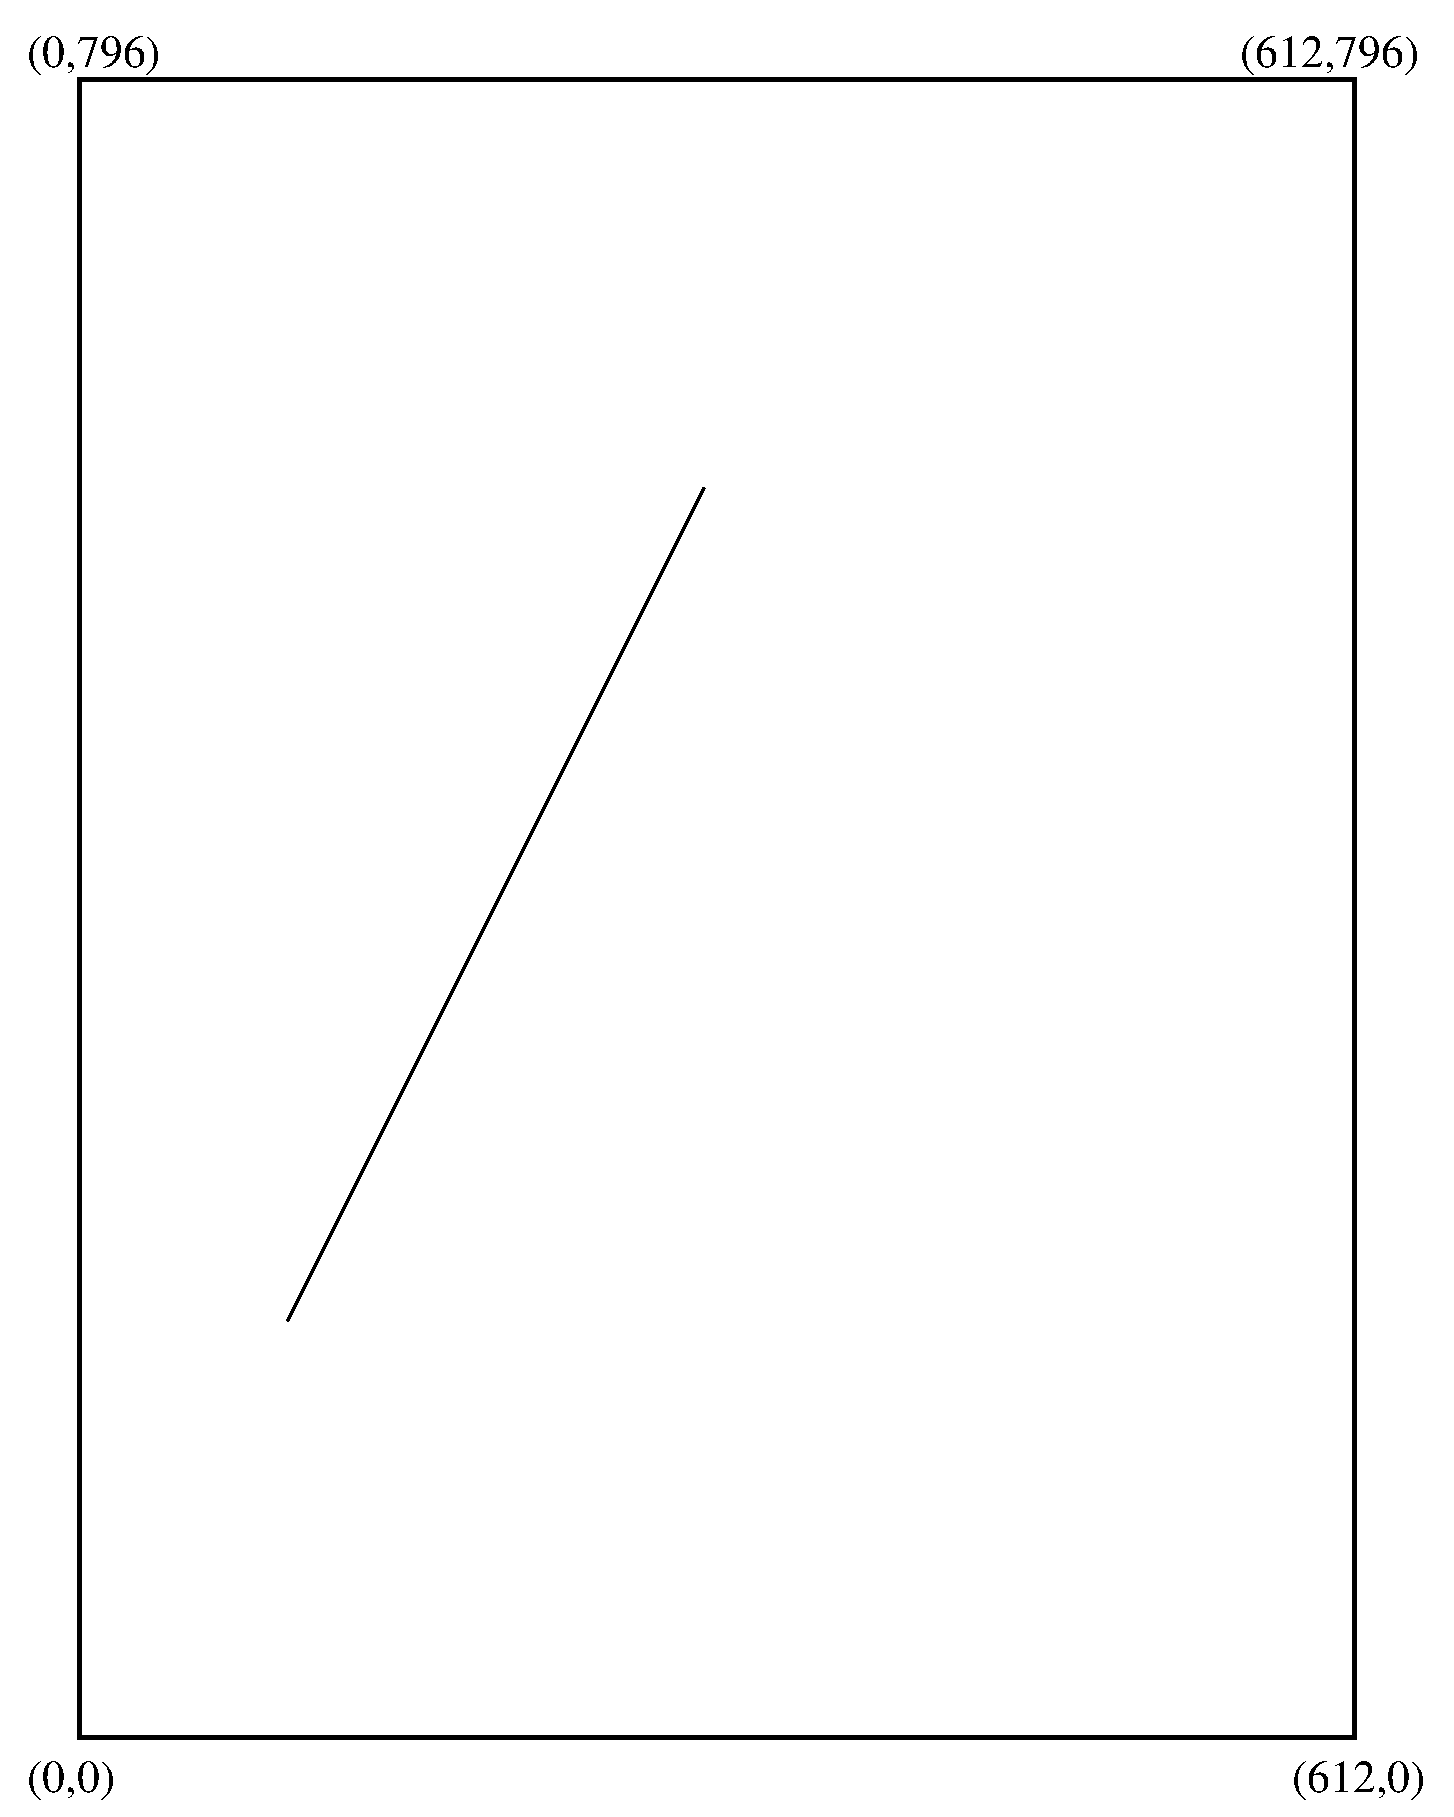
\epsfig{width=2.5in,file=Figures/Postscript-primer/simple-line.eps}
  \end{center} \caption{Simple line rendered by the PostScript
  commands giving in Program \ref{pro:simpleLine} and
  \ref{pro:simpleLineI}.  The surrounding box and corner labels have
  been added for the sake of clarity.}  \label{fig:simpleLine}
\end{figure}

Instead of using the command {\tt lineto} to specify the point to
which we want the line to be drawn, the command {\tt rlineto} can be
used where now the arguments specify the relative movement from the
current point (hence the ``r'' for relative).  The arguments of {\tt
rlineto} specify the relative displacement from the current point.  In
the commands in Program \ref{pro:simpleLine}, the line which was drawn
went $200$ points in the $x$ direction and $400$ points in the $y$
direction from the starting point.  Thus instead of writing {\tt 300
600 lineto}, one could obtain the same result using {\tt 200 400
rlineto}.  PostScript does not care about whitespace and the percent
sign is used to indicate the start of a comment (the interpreter
ignores everything from the percent sign to the end of the line).
Thus, another file which would also yield the output shown in Fig.\
\ref{fig:simpleLine} is shown in Program \ref{pro:simpleLineI}.
(The magic word must appear by itself on the first line of the file.)
\begin{program}
PostScript commands to draw a single tilted line.  Here the {\tt
rlineto} command is used.  The resulting image is identical to the one
produced by Progam \ref{pro:simpleLine} and is shown in Fig.\
\ref{fig:simpleLine}.  \label{pro:simpleLineI}
\codemiddle
\begin{verbatim}
  %!PS
  % tilted line using the rlineto command
  100 200 moveto 300 600 lineto stroke showpage
\end{verbatim}
\end{program}

When creating graphics it is often convenient to redefine the origin
of the coordinate system to a point which is more natural to the
object being drawn.  PostScript allows us to translate the origin to
any point on the page using the {\tt translate} command.  This command
also takes two arguments corresponding to the point in the current
coordinate system where the new origin should be located.  For
example, let us assume we want to think in terms of both positive and
negative coordinates.  Therefore we wish to place the origin in the
middle of the page.  This can be accomplished with the command {\tt
306 396 translate}.  The PostScript commands shown in Program
\ref{pro:transExample} demonstrate the use of the {\tt translate}
command.
\begin{program}
PostScript commands which first translate the origin to the center of
the page and then draw four lines which ``radiate away'' from the
origin.  The corner labels show the corner coordinates after the
translation of the origin to the center of the page.
\label{pro:transExample}
\codemiddle
\begin{verbatim}
  %!PS
  306 398 translate  % translate origin to center of page
   100  100 moveto  50  50 rlineto stroke
  -100  100 moveto -50  50 rlineto stroke
  -100 -100 moveto -50 -50 rlineto stroke
   100 -100 moveto  50 -50 rlineto stroke
  showpage
\end{verbatim}
\end{program}
Program \ref{pro:transExample} yields the results shown in Fig.\
\ref{fig:transExample}.
\begin{figure}
  \begin{center}
  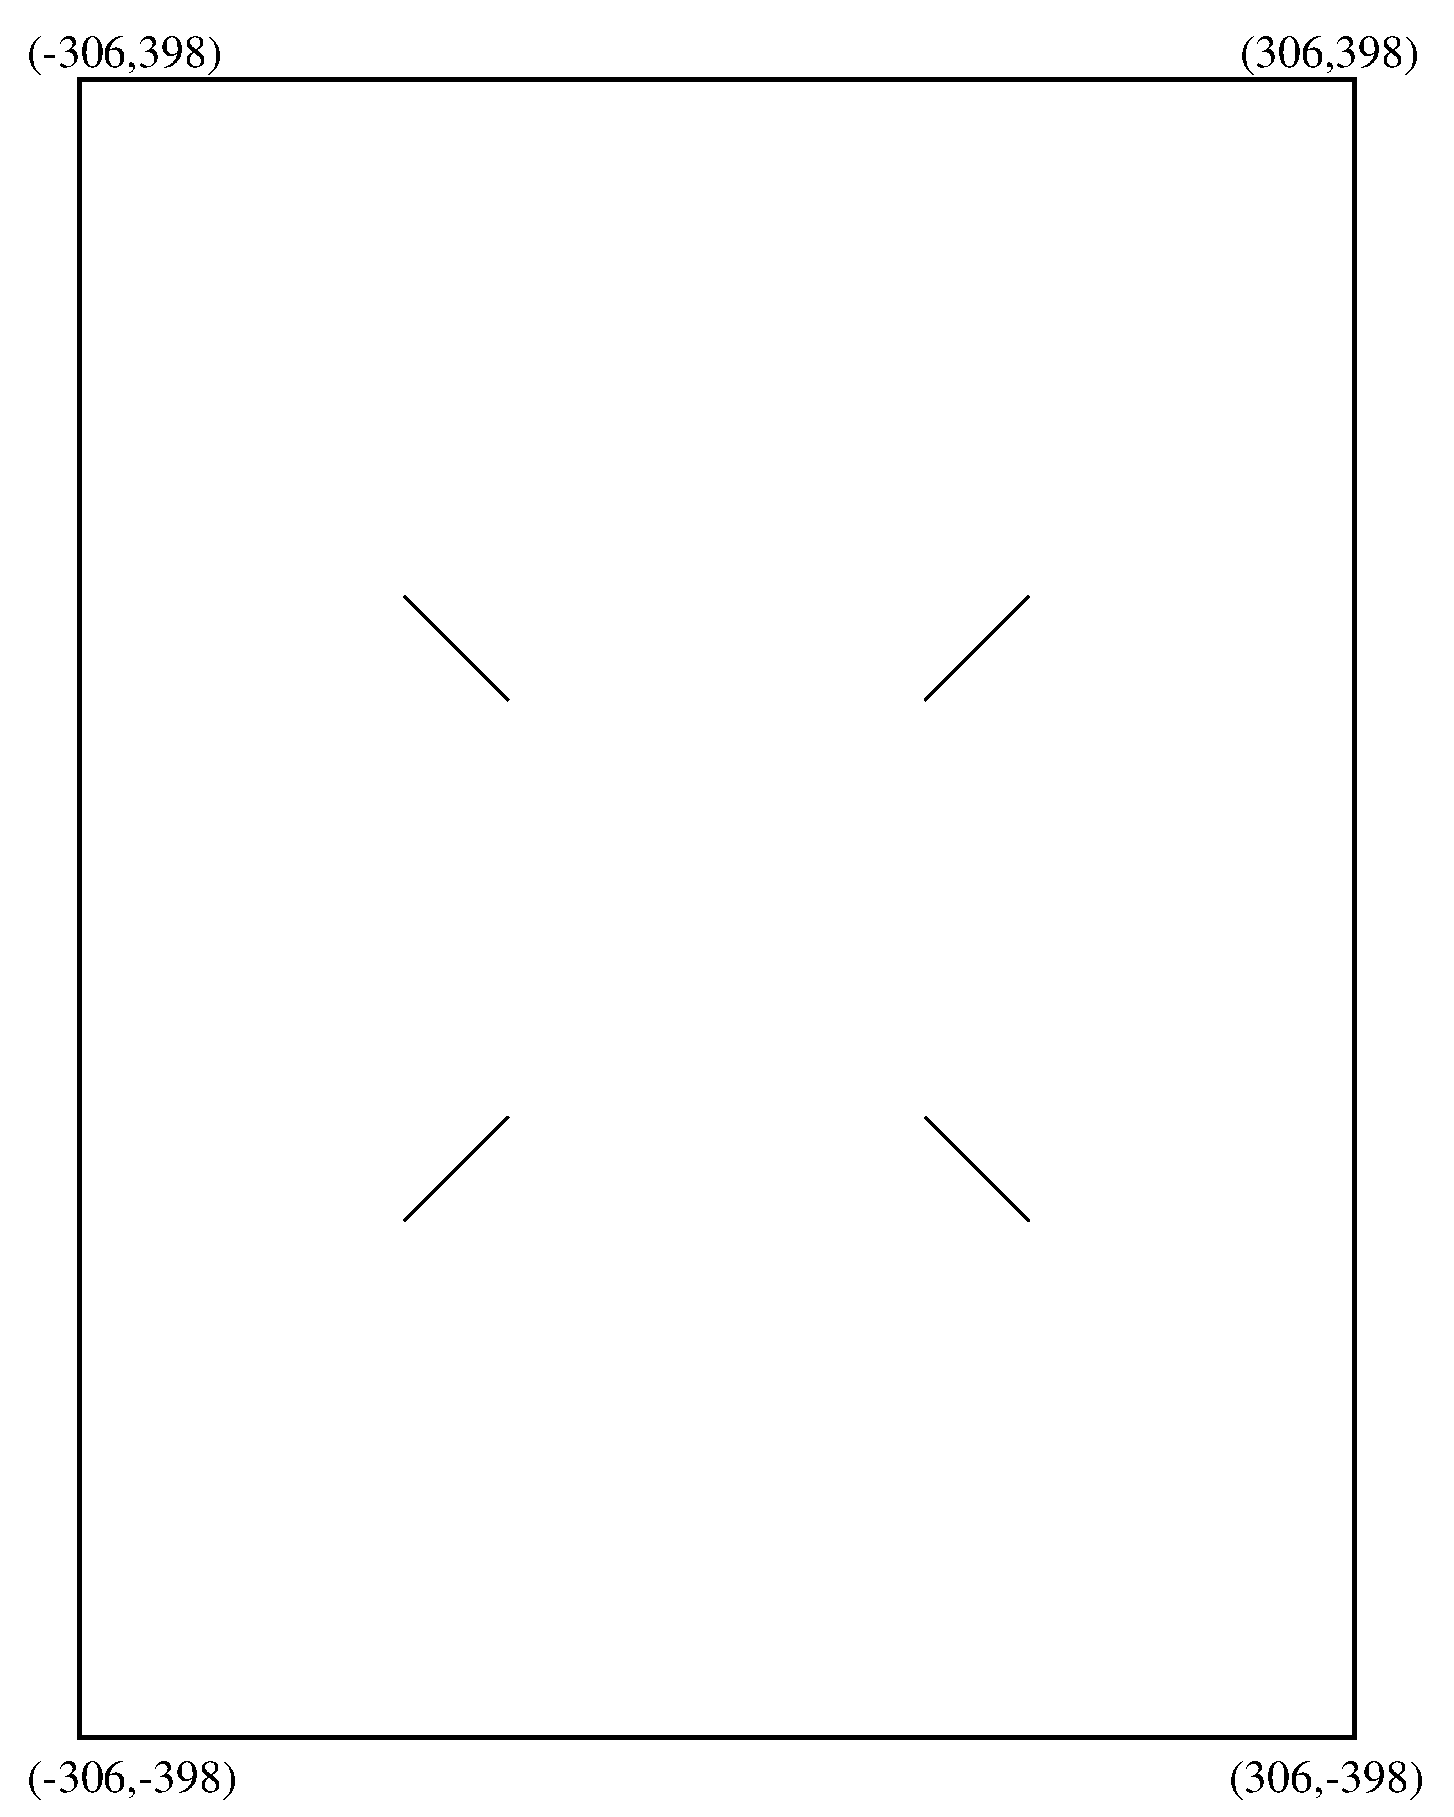
\epsfig{width=2.5in,file=Figures/Postscript-primer/trans-example.eps}
  \end{center} \caption{Output rendered by Program
  \ref{pro:transExample} which translates the origin to the center of the
  page.  This output is also produced by  Program
  \ref{pro:scaleExampleI} and  Program
  \ref{pro:scaleExampleII}.}  \label{fig:transExample}
\end{figure}

As you might imagine, thinking in terms of units of points ($1/72$ of
an inch) is not always convenient.  PostScript allows us to scale the
dimensions by any desired value using the {\tt scale} command.  In
fact, one can use a different scale factor in both the $x$ and the $y$
directions and thus {\tt scale} takes two arguments.  However, we will
stick to using equal scaling in both directions.

In the previous example, all the locations were specified in terms of
multiples of $50$.  Therefore it might make sense to scale the
dimensions by a factor of $50$ (in both the $x$ and $y$ direction).
This scaling should be done {\em after} the translation of the origin.
We might anticipate that the commands shown in Program
\ref{pro:scaleExample} would render the same output as shown in Fig.\
\ref{fig:transExample}.
\begin{program}
PostScript file where the units are scaled by a factor of $50$ in both
the $x$ and $y$ dimensions.  \label{pro:scaleExample}
\codemiddle
\begin{verbatim}
  %!PS
  306 398 translate
  50 50 scale % scale units in x and y direction by 50
   2  2 moveto  1  1 rlineto stroke
  -2  2 moveto -1  1 rlineto stroke
  -2 -2 moveto -1 -1 rlineto stroke
   2 -2 moveto  1 -1 rlineto stroke
  showpage
\end{verbatim}
\end{program}
However this file yields the output shown in Fig.\ \ref{fig:transScale}.
\begin{figure}
  \begin{center}
  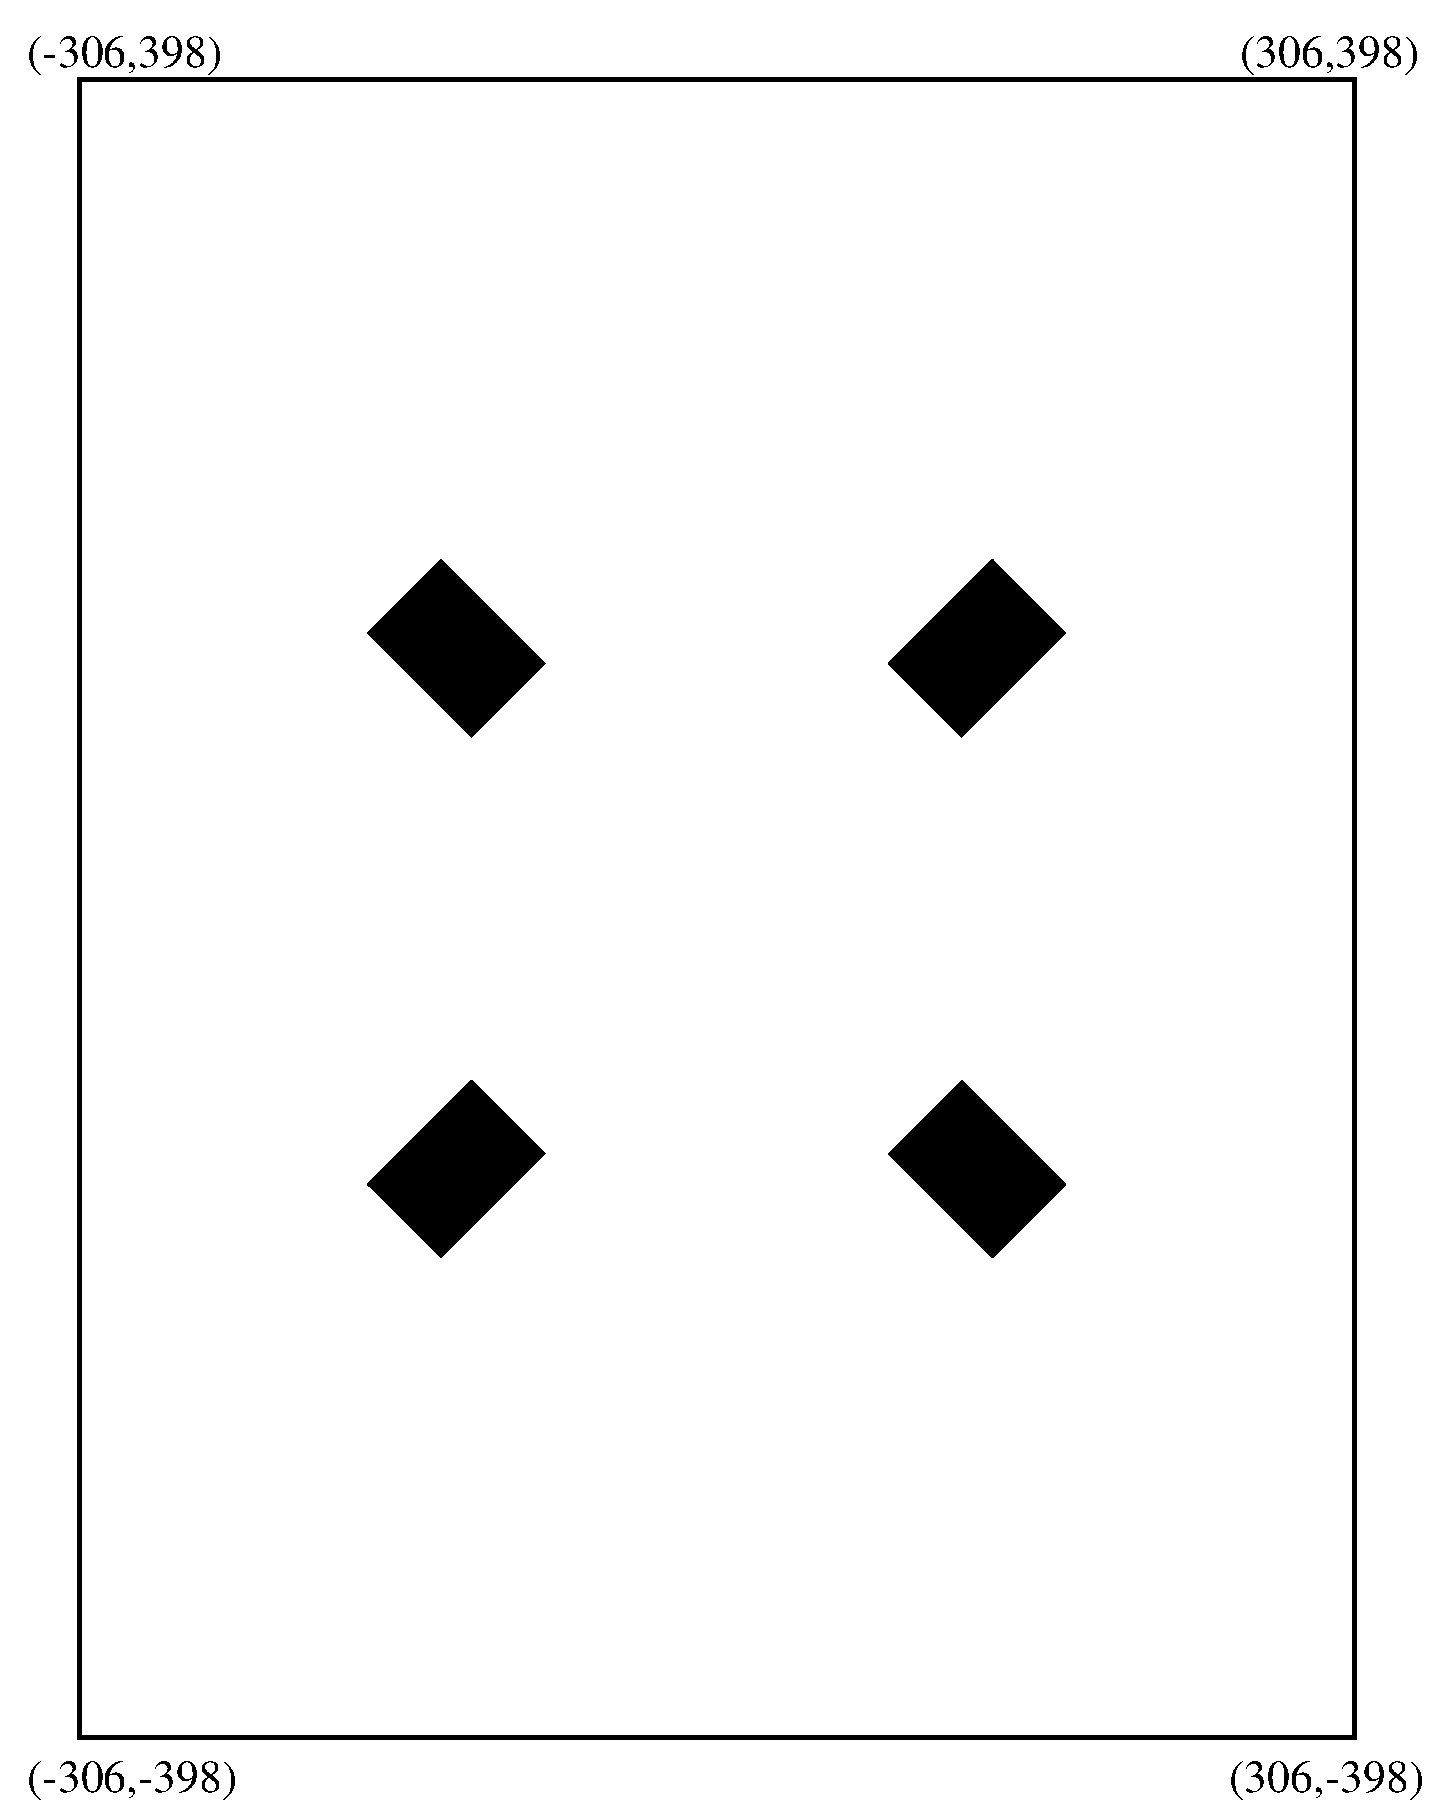
\epsfig{width=2.5in,file=Figures/Postscript-primer/trans-scale.eps}
  \end{center} \caption{Output rendered by Program
  \ref{pro:scaleExample} which scales the units by $50$.}
  \label{fig:transScale}
\end{figure}
Note that the lines which radiate from origin are now much thicker.
In fact, they are $50$ times thicker than they were in the previous
image.  By default, a line in PostScript has a thickness of unity
i.e., one point.  The {\tt scale} command scaled the line thickness
along with all the other dimensions so that now the line thickness is
$50$ points.

Although we have only given integer dimensions so far, as far as
PostScript is concerned all values are actually real numbers (i.e.,
floating-point numbers).  We can control the line thickness with the
{\tt setlinewidth} command which takes a single argument.  If we want
the line thickness still to be one point, the line thickness should be
set to the inverse of the scale factor, i.e., $1/50=0.02$.  Also, it
is worth noting that the stroke command does not have to be given
after each drawing command.  We just have to ensure that it is given
before the end of the file (or before the line style changes to
something else).  Thus, a PostScript file which scales the dimensions
by $50$ and produces the same output as shown in Fig.\
\ref{fig:transExample} is shown in Program \ref{pro:scaleExample}
\begin{program}
PostScript file where the units are scaled by a factor of $50$ and the
line thickness is corrected to account for this scaling.  Note that a
single {\tt stroke} command is given.
\label{pro:scaleExampleI}
\codemiddle
\begin{verbatim}
  %!PS
  306 398 translate
  50 50 scale
  0.02 setlinewidth  % correct line thickness to account for scaling
   2  2 moveto  1  1 rlineto
  -2  2 moveto -1  1 rlineto
  -2 -2 moveto -1 -1 rlineto
   2 -2 moveto  1 -1 rlineto stroke
  showpage
\end{verbatim}
\end{program}

PostScript permits the use of named variables and, as we shall see,
named procedures.  This is accomplished using the {\tt def} command
which takes, essentially, two arguments: the first being the literal
string which is the variable or procedure name and the second being
the value or procedure (where the procedure would be enclosed in
braces).  A literal string is a backslash character followed by the
string.  For example, the following sets the variable {\tt scalefactor} to
$50$:
\begin{verbatim}
  /scalefactor 50 def
\end{verbatim}
After issuing this command, we can use {\tt scalefactor} in place of
$50$ everywhere in the file.

The PostScript language includes a number of mathematical functions.
One can add using {\tt add}, subtract using {\tt sub}, multiply using
{\tt mul}, and divide using {\tt div}.  Each of these functions takes
two arguments consistent with an RPN calculator.  To calculate
the inverse of $50$, one could issue the following command:
\begin{verbatim}
  1 50 div
\end{verbatim}
This places $1$ on the stack, then $50$, and then divides the two.  The
result, $0.02$, remains at the top of the stack.

The program shown in Program \ref{pro:scaleExampleII} uses the {\tt
def} and {\tt div} commands and is arguably a bit cleaner and better
self-documenting than the one shown in Program
\ref{pro:scaleExampleI}.  Program \ref{pro:scaleExampleII} also
produces the output shown in Fig.\ \ref{fig:transExample}.  
\begin{program}
PostScript file which uses the {\tt def} command to define a
scale-factor which is set to $50$.  The inverse of the scale-factor is
obtained by using the {\tt div} command to divide $1$ by the scale-factor.
\label{pro:scaleExampleII}
\codemiddle
\begin{verbatim}
  %!PS
  306 398 translate
  % define "scalefactor" to be 50
  /scalefactor 50 def
  % scale x and y directions by the scale factor
  scalefactor scalefactor scale
  % set line width to inverse of the scale factor
  1 scalefactor div setlinewidth
   2  2 moveto  1  1 rlineto
  -2  2 moveto -1  1 rlineto
  -2 -2 moveto -1 -1 rlineto
   2 -2 moveto  1 -1 rlineto stroke
  showpage
\end{verbatim}
\end{program}

The {\tt arc} command takes five arguments: the $x$ and $y$ location
of the center of the arc, the radius of the arc, and the angles (in degrees) at
which the arc starts and stops.  For example, the following command
would draw a complete circle of radius $0.5$ about the point $(2,2)$:
\begin{verbatim}
  2 2 0.5 0 360 arc stroke
\end{verbatim}
Let us assume we wish to draw several circles, each of radius $0.5$.
We only wish to change the center of the circle.  Rather than
specifying the {\tt arc} command each time with all its five
arguments, we can use the {\tt def} command to make the program more
compact.  Consider the program shown in Program
\ref{pro:circleExample}.  Here the {\tt def} command is used to say
that the literal {\tt circle} is equivalent to {\tt 0.5 0 360 arc
stroke}, i.e., three of the arguments are given to the {\tt arc}
command---one just has to provide the two missing arguments which are
the $x$ and $y$ location of the center of the circle.  The output
produced by this program is shown in Fig.\
\ref{fig:circleExample}.
\begin{program}
PostScript file which renders the output shown in Fig.\
\ref{fig:circleExample}.
\label{pro:circleExample}
\codemiddle
\begin{verbatim}
  %!PS
  306 398 translate
  /scalefactor 50 def
  scalefactor scalefactor scale
  1 scalefactor div setlinewidth
  /circle {0.5 0 360 arc stroke} def
   2  2 circle
  -2  2 circle
  -2 -2 circle
   2 -2 circle
  showpage
\end{verbatim}
\end{program}

\begin{figure}
  \begin{center}
  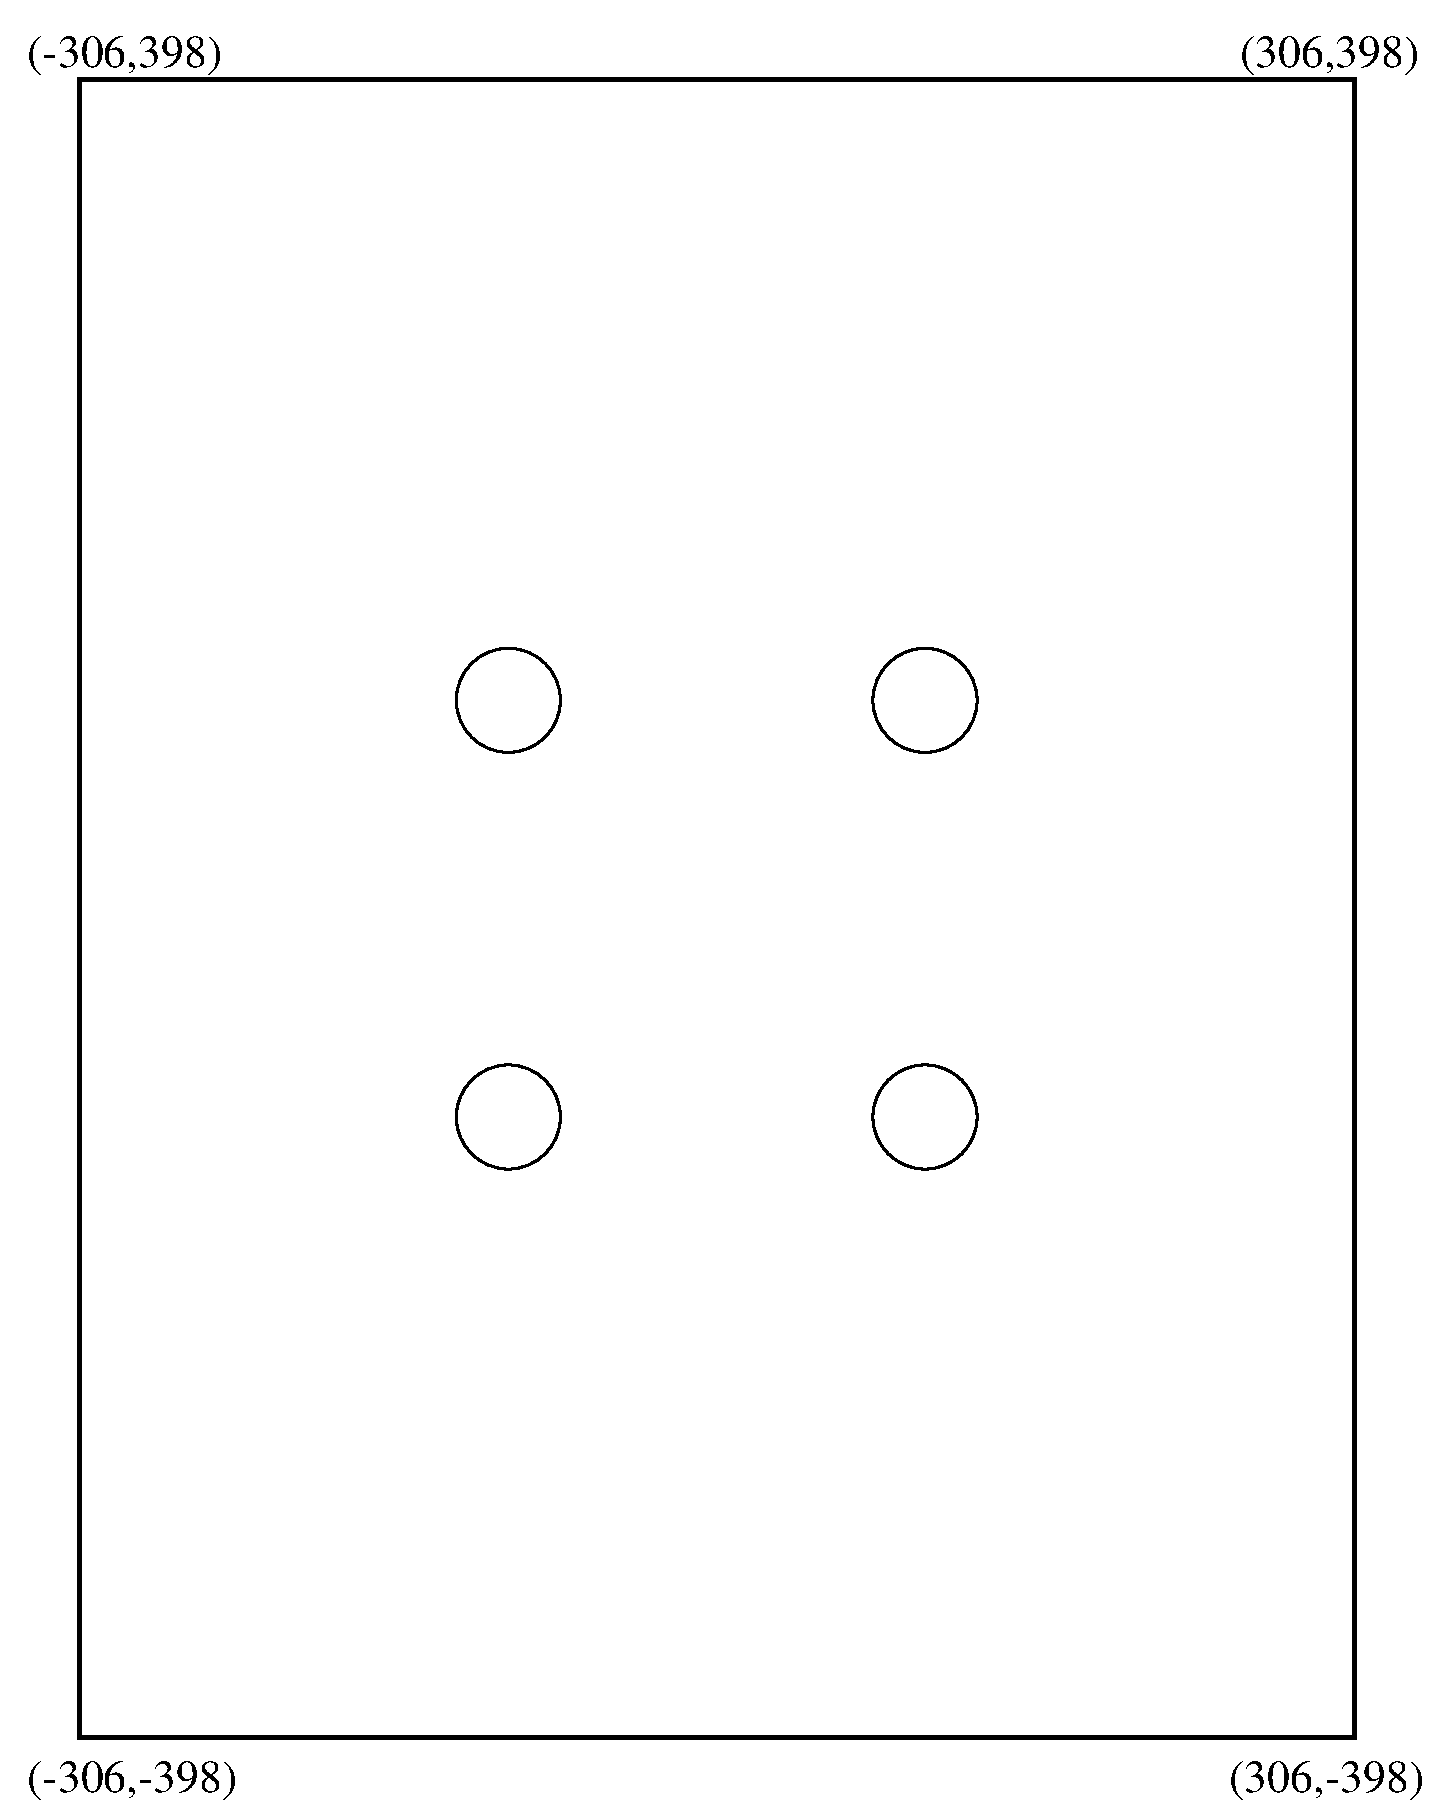
\epsfig{width=2.5in,file=Figures/Postscript-primer/circle.eps}
  \end{center} \caption{Output rendered by Program
  \ref{pro:circleExample}.}
  \label{fig:circleExample}
\end{figure}

In addition to {\tt stroke}-ing a path, PostScript allows paths to be
{\tt fill}-ed using the fill command.  So, instead of drawing a line
around the perimeter of the circles shown in Fig.\
\ref{fig:circleExample}, one can obtain filled circles by issuing the
{\tt fill} command instead of the {\tt stroke} command.  Program
\ref{pro:circleExampleI} and the corresponding output shown in Fig.\
\ref{fig:circleExampleI} illustrate this.
\begin{program}
PostScript file which defines a {\tt stroke}-ed and {\tt fill}-ed circle.
The corresponding output is shown in Fig.\ \ref{fig:circleExampleI}.
\label{pro:circleExampleI}
\codemiddle
\begin{verbatim}
  %!PS
  306 398 translate
  /scalefactor 50 def
  scalefactor scalefactor scale
  1 scalefactor div setlinewidth
  /circle {0.5 0 360 arc stroke} def
  /circlef {0.5 0 360 arc fill} def
   2  2 circlef
  -2  2 circle
  -2 -2 circlef
   2 -2 circle
  showpage
\end{verbatim}
\end{program}

\begin{figure}
  \begin{center}
  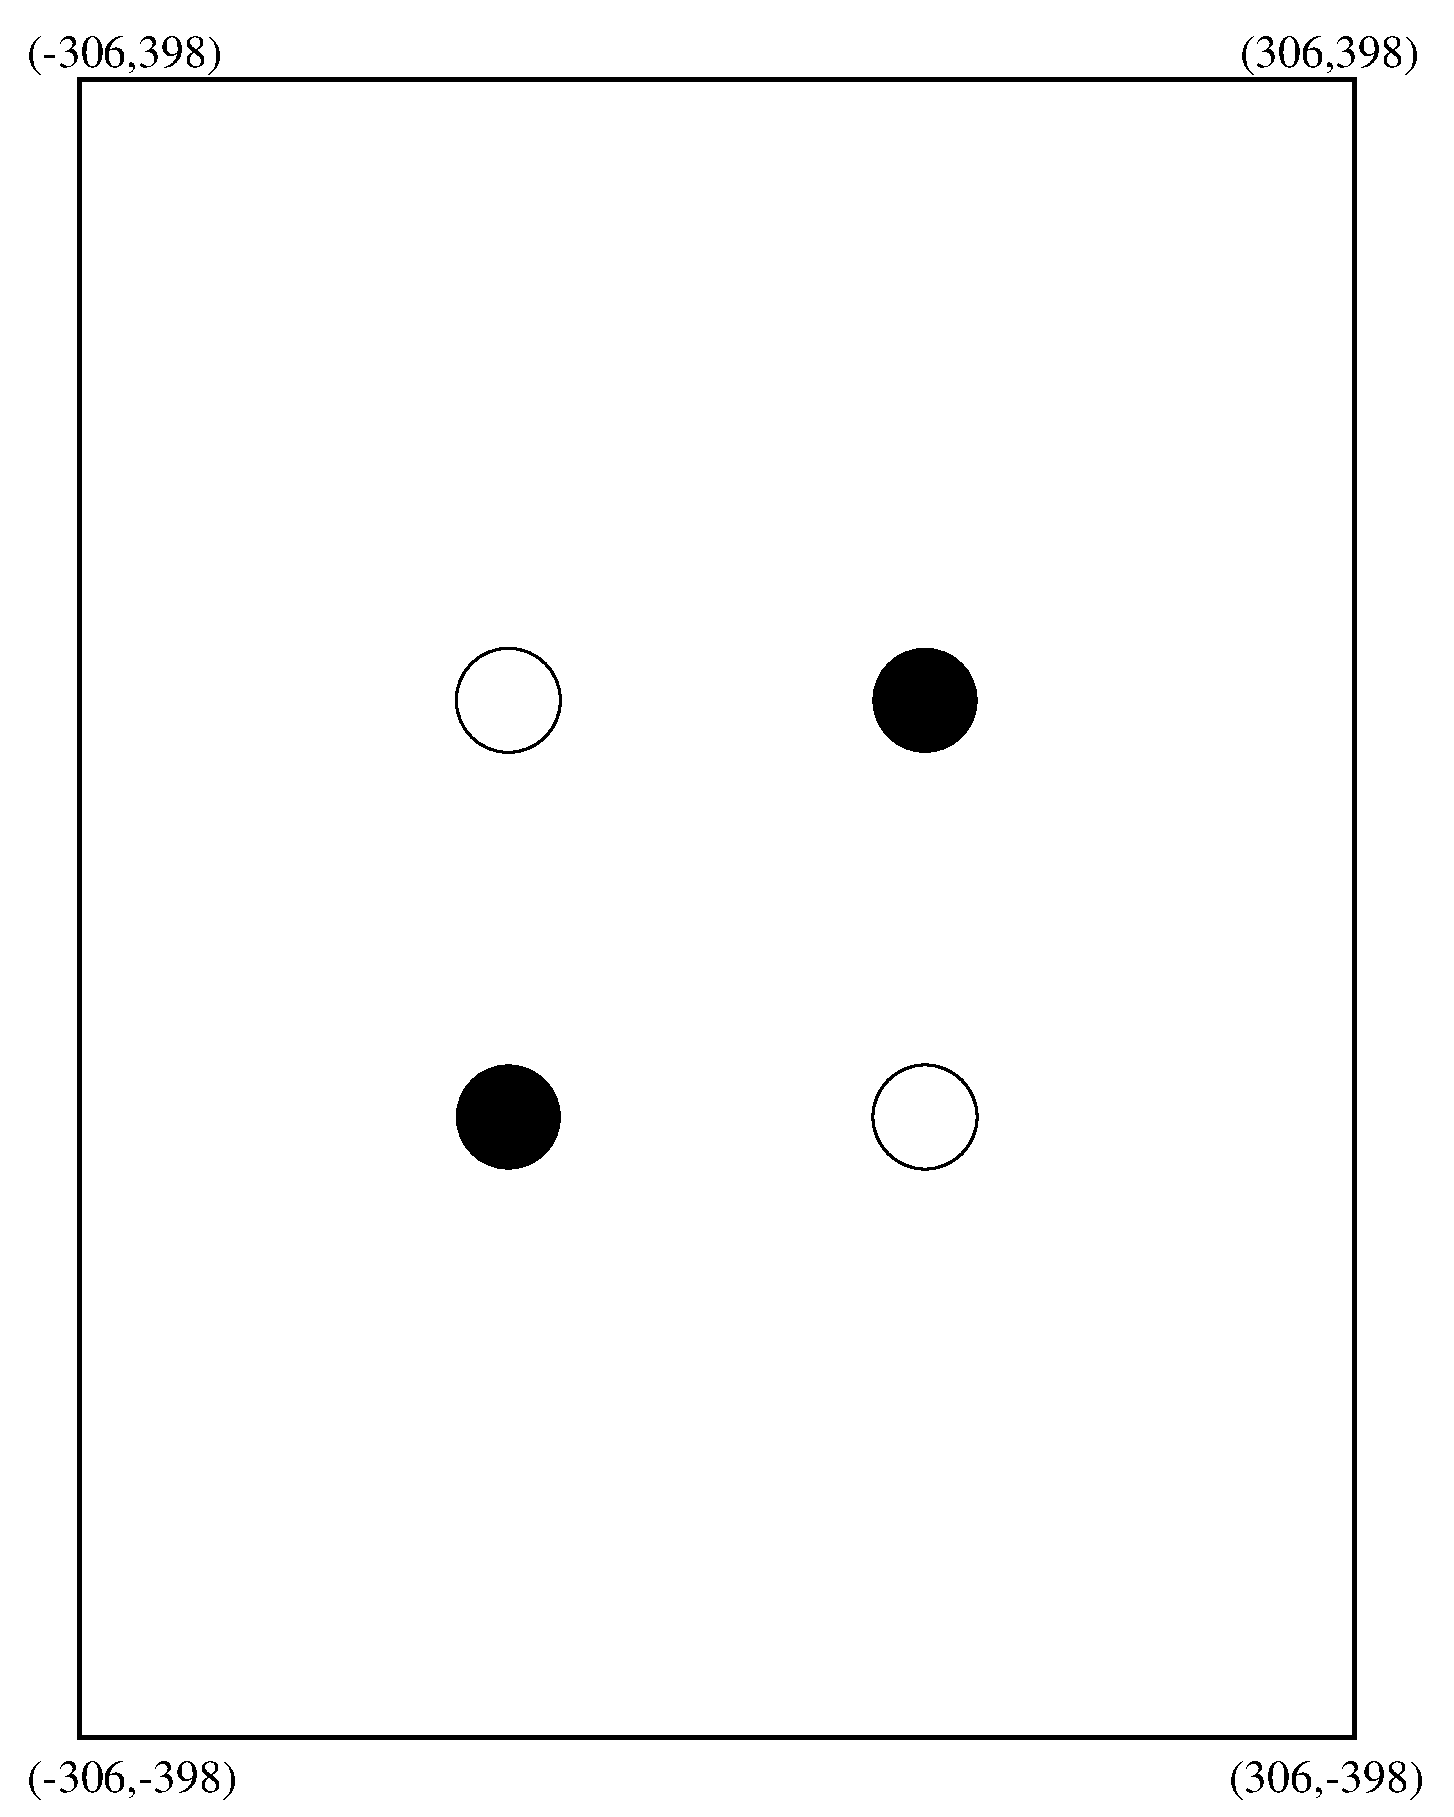
\epsfig{width=2.5in,file=Figures/Postscript-primer/circleI.eps}
  \end{center} \caption{Output rendered by Program
  \ref{pro:circleExampleI}.}
  \label{fig:circleExampleI}
\end{figure}

The PostScript commands we have considered are shown in Table
\ref{tab:postscript}.
\begin{table}
\begin{tabular}{ll}
Command & Description \\ \hline
$x$ $y$ {\tt moveto} &  move current point to $(x,y)$ \\
$x$ $y$ {\tt lineto} & draw a line from current point to $(x,y)$ \\
$\delta_x$ $\delta_y$ {\tt rlineto}&
 from current point draw a line over $\delta_x$ and up $\delta_y$ \\
$x$ $y$ {\tt translate} & translate the origin to the point $(x,y)$ \\
$s_x$ $s_y$ {\tt scale} & scale $x$ and $y$ coordinates by $s_x$ and
  $s_y$ \\
{\tt stroke} & ``apply ink'' to a previously defined path\\
{\tt fill}   & fill the interior of a previously defined path\\
$w$ {\tt setlinewidth} & set the line width to $w$\\
$d_1$ $d_2$ {\tt div} & calculate $d_1/d_2$;
            result is placed at top of stack \\
$x_c$ $y_c$ $r$ $a_1$ $a_2$ {\tt arc} & draw an arc of radius $r$
centered at $(x_c,y_c)$ \\
  & starting at angle $a_1$ and ending at angle $a_2$ (degrees) \\
/{\em literal} \{{\em definition}\} {\tt def} & define the {\em
literal} string to have the given {\em definition}; \\
  & braces are needed if the definition contains any whitespace
\end{tabular}
\caption{An assortment of PostScript commands and their arguments.} \label{tab:postscript}
\end{table}

Instead of using an editor to write a PostScript file directly, we can
use another program to generate the PostScript file for us.
Specifically, let us consider a C program which generates a PostScript
file.  This program is supposed to demonstrate how one could use
PostScript to display a particular aspect of an FDTD grid.  For
example, let us assume we are using a TM$^z$ grid which is $21$ cells
by $21$ cells.  There is a PEC cylinder with a radius of $5$ which is
centered in the grid.  We know that the $E_z$ nodes which fall within
the cylinder should be set to zero and this zeroing operation would be
done with a for-loop.  However, precisely which nodes are being set to
zero?  The code shown in Program \ref{pro:gridDisplay} could be
incorporated into an FDTD program.  This code produces the PostScript
output file {\tt grid.ps} which renders the image shown in Fig.\
\ref{fig:gridDisplay}.  The first several lines of the file {\tt
grid.ps} are shown in Fragment \ref{frag:gridDisplay}.
\begin{program}
C program which generates a PostScript file.  The file draws either a
cross or a filled circle depending on whether a node is outside or
inside a circular boundary, respectively.  The rendered image is shown
in Fig.\ \ref{fig:gridDisplay}.
\label{pro:gridDisplay}
\codemiddle
\begin{lstlisting}
/* C program to generate a PostScript file which draws a cross
 * if a point is outside of a circular boundary and draws a
 * filled circle if the point is inside the boundary.
 */

#include <stdio.h>
#include <math.h>

int is_inside_pec(double x, double y);

int main() {
  int m, n;

  FILE *out;

  out = fopen("grid.ps","w");  // output file is "grid.ps"

  /* header material for PostScript file */
  fprintf(out,"%%!PS\n"
          "306 396 translate\n"
          "/scalefactor 20 def\n"
          "scalefactor scalefactor scale\n"
          "1 scalefactor div setlinewidth\n"
          "/cross {moveto\n"
          "         -.2 0 rmoveto .4 0 rlineto\n"
          "         -.2 -.2 rmoveto 0 .4 rlineto stroke} def\n"
          "/circle {.2 0 360 arc fill} def\n"
          );

  for (m=-10; m<=10; m++)
    for (n=-10; n<=10; n++)
      if (is_inside_pec(m,n)) {
        fprintf(out,"%d %d circle\n",m,n);
      } else {
        fprintf(out,"%d %d cross\n",m,n);
      }

  fprintf(out,"showpage\n");

  return 0;
}

/* Function returns 1 if point (x,y) is inside a circle (or on
 * the perimeter of circle) and returns 0 otherwise.
 */
int is_inside_pec(double x, double y) {
  double radius = 5.0;

  return x*x + y*y <= radius*radius;
}
\end{lstlisting}
\end{program}

\begin{figure}
  \begin{center}
  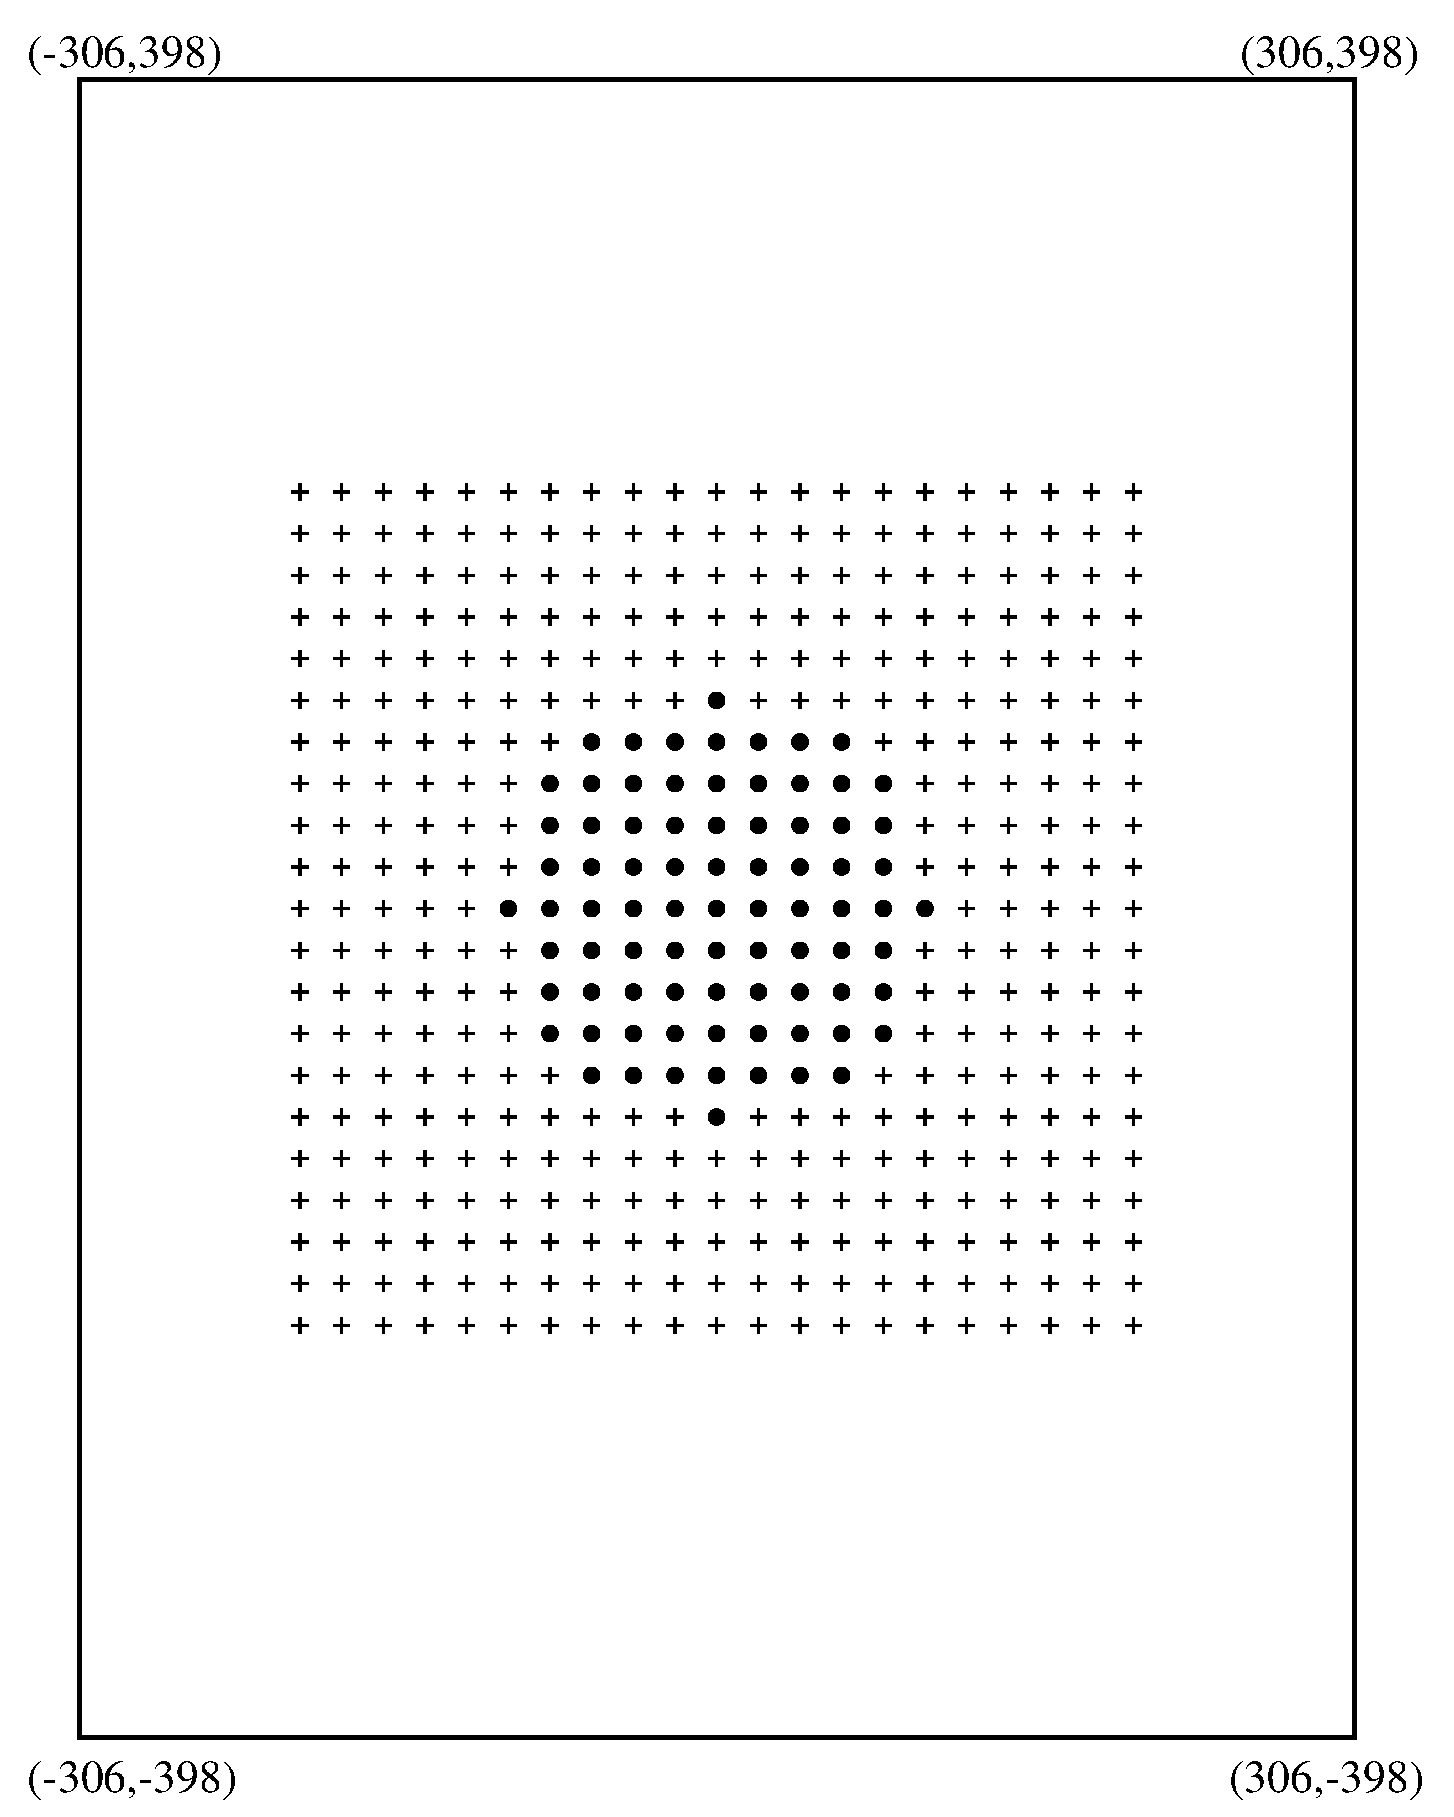
\epsfig{width=3.5in,file=Code/Postscript-primer/grid.eps}
  \end{center} \caption{Grid depiction rendered by the file {\tt
  grid.ps} which is produced by Program
  \ref{pro:gridDisplay}.  Crosses corresponds to nodes which are outside
  a circular boundary of radius $5$.  Filled circles correspond to
  nodes inside the boundary (or identically on the perimeter of the
  boundary).}
  \label{fig:gridDisplay}
\end{figure}

\begin{fragment}
First several lines of the file {\tt grid.ps} which is produced by
Program \ref{pro:gridDisplay}.
\label{frag:gridDisplay}
\codemiddle
\begin{verbatim}
%!PS
306 396 translate
/scalefactor 20 def
scalefactor scalefactor scale
1 scalefactor div setlinewidth
/cross {moveto
         -.2 0 rmoveto .4 0 rlineto
         -.2 -.2 rmoveto 0 .4 rlineto stroke} def
/circle {.2 0 360 arc fill} def
-10 -10 cross
-10 -9 cross
-10 -8 cross
-10 -7 cross
-10 -6 cross
    .
    .
    .
\end{verbatim}
\end{fragment}
